%!TEX root = ../paper.tex
%!TEX encoding = UTF-8 Unicode

\section{Background}\label{sec:background}
%Como e que as apliccaoes sao recuperadas, de modo generico e com o related work incluido
%and Related Work

This section formalizes the distinct approaches to perform intrusion recovery and presents the main related work. 

An application execution is modeled as a set of actions $A$ on a set of objects $O$. Actions are described by operations (read, write, others more complex), the value(s) read/written, and a timestamp (which defines the order of the actions). Each object has a state (or value) and a set of operations that can modify it. We specify $A_{intrusion}$ as the subset of actions of $A$ whereby the attacker compromises the application during the intrusion, $A_{after}$ as the subset of actions that began after the intrusion began (including the first action of the intrusion), and $A_{legal}$ as the subset of legitimate actions in $A$, i.e., $A_{legal} = A \backslash A_{intrusion}$.

A recovery service aims to set the state of the objects that compose an application to $O_{recovered}$ at the end of a recovery process. The set $O_{recovered}$ shall be composed of objects as if their state was defined by a set of legitimate actions $A_{recovered}$. Objects of the subset $O_{recovered}$ represent an intrusion-free and consistent state. A state is said to be \textit{consistent} if it is valid according to the application specification. A state is said to be \textit{intrusion-free} if it is created only by legitimate actions. If the application respects the specification (correctness), then changing from $O$ to $O_{recovered}$ performs service restoration \cite{Aviz}, i.e., restores the application service to a correct behavior. %mpc: esta ultima frase nao parece muito bem

A backup mechanism is a basic recovery service that sets the objects to the state they had before the intrusion began. This new state $O_{recovered}$ excludes the state set by the attacker's actions ($A_{intrusion}$), but also the state set by the legitimate actions performed after that point ($A_{legal}$). This second aspect is undesirable in many systems, so intrusion recovery systems avoid it.

We define the set of \textit{tainted} actions, $A_{tainted}$, and the set of tainted objects, $O_{tainted}$, at a certain instant in the following way: if an action belongs to $A_{intrusion}$, then it belongs to $A_{tainted}$; if an object belongs to $O_{intrusion}$ then it belongs to $O_{tainted}$; if an action in $A_{legal}$ reads an object in $O_{tainted}$, then that action belongs to $A_{tainted}$; if an action in $A_{tainted}$ writes a value in an object in $O_{legal}$, then that object belongs to $O_{tainted}$  (Figure \ref{img:sets}). Therefore, $A_{tainted}$ includes $A_{intrusion}$ but typically also actions from $A_{legal}$ that were contaminated by corrupted state. \LONG{Similarly, $O_{tainted}$ includes $O_{intrusion}$ but typically also objects from $O_{legal}$. Then, the set of object values written only by non-malicious actions is not the same as the set of objects obtained after removing the objects written by malicious and tainted actions. In other words,} Therefore, to remove the state compromised by tainted actions is necessary but not enough to obtain the state of the set of objects that would be produced only by legitimate actions.


Some intrusion recovery systems \cite{taser,itdb,phoenix} attempt to obtain $O_{recovered}$ by removing 
the state of the objects of $O_{tainted}$ from the current state $O$. To do so, the value of each object in $O_{tainted}$ is \textit{replaced} by a previous value. These systems keep the objects written by legitimate actions, $O_{legal}$, unmodified.
%mpc: falta explicar isto um pouco melhor e discutir limitacoes, comparando com este trabalho. REVER COM O MATERIAL DOS PAPERS PARA NAO DIZER ALGO ERRADO

\begin{figure}
  \centering
  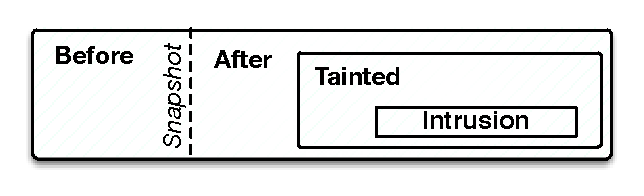
\includegraphics[width=60mm]{images/sets}
  \caption{Set of actions: A set of actions is splitted by the snapshot into \textit{before} and \textit{after} snapshot. A subset of actions of \textit{after} is \textit{tainted} by a subset of malicious actions of an \textit{intrusion}.}
  \label{img:sets}
\end{figure}

%mpc: o proximo parag. esta' algo complicado; devia ser escrito de forma mais directa

A different approach consists generically in replaying actions. \LONG{Let us motivate this possibility with a non-practical case.} Consider a hypothetical application execution at a certain point in time, after the intrusion, where the actions in $A$ are replaced by those in $A_{recovered} = A \backslash A_{intrusion} = A_{legal}$, i.e., the intrusion actions $A_{intrusion}$ are not executed. 
If the state was rewind to the beginning of the application execution and only the actions in $A_{recovered}$ were re-executed, the application would be intrusion free as 
$A \cap A_{intrusion} = \emptyset \implies D_{intrusion} = \emptyset, A_{tainted} = \emptyset \implies D_{tainted} = \emptyset$. 
Since the malicious actions were removed, the state, $O$, would not have values imposed by $A_{intrusion}$. 
For this reason, the sequence of tainted actions $A_{tainted}$ would be empty. 
The set of tainted actions on the non-hypothetical application execution, which includes $A_{intrusion}$, would read different values and have a different execution if $A_{intrusion}$ was empty. 
Therefore, if $A_{intrusion}$ and $O_{intrusion}$ are removed, then $A_{tainted}$ should be \emph{replayed} because the actions of $A_{tainted}$ are not contaminated by malicious data during their re-execution. The replay process restores the application to a correct state $O_{recovered}$, which is intrusion-free.

That generic approach is unfeasible without the use of snapshots.
The sequence of actions performed before the intrusion $A_{before} = A \backslash A_{after}$ can be long and each action takes non-null time to execute, so replaying $A_{before}$ may be unfeasible. Moreover, a log of all the actions executed may be too large.
We define the subsets $O_{snapshot}(t)$ and $A_{snapshot}(t) : A_{snapshot}(t) \subset A$ as the subsets of objects and actions executed before the begin of a snapshot operation at instant \textit{t}. 
%The snapshot operation copies the value of the object immediately or on the next write operation. 
If the intrusion happens after $t$, then $A_{after} \cap A_{snapshot}(t) = \emptyset \implies (A_{intrusion} \cup A_{tainted}) \cap A_{snapshot}(t) = \emptyset$, i.e., the snapshot is not affected by the intrusion. For that reason, the service can replay only $A \backslash A_{snapshot}(t) \backslash A_{intrusion}$ using the object set $O_{snapshot}$ as base. 

There are two distinct replay approaches to update the set of object $O$ to $O_{recovered}$, 
%because of changes in the execution of $A_{tainted}$
selective replay and full replay. 
A \textit{version} is a snapshot of a single object value at an instant $t$. Versions can be recorded with the sequence of actions that write the objects before the instant $t$.
The \textit{selective replay} approach \cite{taser,warp,goel} loads only the versions of the tainted objects, $O_{tainted}$ previous to the intrusion, instead of loading a previous version of every object. Then, it replays only the legitimate actions, which were tainted, $A_{tainted} \backslash A_{intrusion}$, to update the objects in $O$. The state of the objects in $O_{legal} \backslash D_{tainted}$ remains unmodified. 
The other approach, \textit{full replay} \cite{undoForOperators}, loads a snapshot previous to the intrusion moment and replays every action in $A \backslash A_{snapshot}(t) \backslash A_{intrusion}$. This approach is slightly simpler than the other, but in general takes longer to execute. 

%mpc: movi a definicao de version para o parag anterior porque fazia la' falta
%A version is a snapshot of a single object value before the instant t. They can be recorded with the sequence of actions that read or write them before the instant t. We define a compensating action as an action that reverts the effects of a original action, for instance writing a previous value. A compensation process can obtain a previous snapshot or version. For this propose, we define the sequence Acompensation(t) as the compensation of Aposteriori(t), the sequence of actions after instant t. The compensation process applies the sequence of compensating actions Acompensation(t) on the current version of the objects, in reverse order, to obtain a previous snapshot or version.


\hl{o proximo paragrafo resume todo o processo de replay mas acho que poderia ser tirado porque vai sendo explicado ao longo do paper}
Recovery services have two distinct phases: \textit{record phase} and \textit{recovery phase}. The record phase is the service usual state where the application is running and the service records the application actions. In order to perform replay, the application actions do not need to be idempotent but their re-execution must be deterministic (given the same initial state they produce the same final state). The record phase should record the actions input and the value of every non-deterministic behavior to turn their re-execution into a deterministic process. The recovery phase can have three phases: determining the affected actions and/or objects, removing these effects, and replaying the actions necessary to recover a consistent state. In this paper we present a recovery service that supports \textit{runtime recovery}, i.e., that does not cause application downtime because the record and recovery phases can occur simultaneously.

\hl{este explica o dependency graph. ou o related work sai e vem para aqui ou entao nao vale a pena ter um pagrafo a falar disto quando ha uma seccao}
Most intrusion recovery services record both the actions and  the objects they accessed  \cite{goel,itdb,warp}. Since the actions read and write objects from a shared set of objects $O$, we can establish dependencies between actions. Dependencies can be visualized as an \textit{action dependency graph} or an \textit{object dependency graph}. The nodes of an action dependency graph represent actions and the edges indicate dependencies though shared objects. An object dependency graph establishes dependencies between objects through actions. Dependency graphs have been used to order the re-execution of actions \cite{undoForOperators}, get the sequence of actions affected by an object value change \cite{warp}, get the sequence of actions tainted by an intrusion \cite{goel} or resolve the set of objects and actions that caused the intrusion using a set of known tainted objects \cite{backtracker}. 

%A \textit{taint algorithm} aims to define the tainted objects $O_{tainted}$ from a set of malicious actions $A_{intrusion}$ or objects $O_{intrusion}$ using a dependency graph. This method is used by selective replay approaches. The \textit{taint propagation via replay} \cite{retro} algorithm begins with the set $O_{tainted}$ determined by the base taint algorithm \hl{o que significa?} and expands the set \hl{o que significa?} $O_{tainted}$. It is used to restore the values of $O_{intrusion} \cup D_{tainted}$ and to replay only the legal actions that output $O_{intrusion} \cup D_{tainted}$ during the first execution. Then it replays the actions dependent from $O_{intrusion} \cup D_{tainted}$, updating their output objects. While the forward actions have different input, they are also replayed and their outputs are updated. 

Dependencies are established during the record phase or at recovery time using the objects and actions. The level of abstraction influences the record technique and the dependency extraction method. The abstraction level defines the recoverable intrusions: operating system \cite{taser,retro}, database \cite{itdb,phoenix}, and application \cite{goel,warp,aire}. In the next sections, we present Shuttle, an intrusion recovery service which recovers from intrusions using the dependencies established at database and application level.
